\documentclass[a4paper, 12pt, answers]{exam}
\usepackage[T1]{fontenc}
\usepackage{amsmath}
\usepackage{amssymb}
\usepackage{enumerate}
\usepackage{bm}
\usepackage{advdate}
\usepackage{datetime}
\usepackage[mathcal]{eucal}
\usepackage{dsfont}
\usepackage[numbered,framed]{matlab-prettifier}
\usepackage{tkz-euclide}
\usepackage[colorlinks,urlcolor=blue]{hyperref}
\usepackage{graphicx}

\usetkzobj{all}
\usepackage{url}
\newdate{issuedate}{22}{11}{2019}
\newdate{duedate}{8}{12}{2019}


\usepackage[noend]{algpseudocode}
\usepackage{algorithmicx,algorithm}

% \newcommand{\duedate}[1][14]{%
% \begingroup
% \AdvanceDate[#1]%
% \today%
% \endgroup
% }%

%% Definitions for Learning from Data
%% UPDATE: October 8, 2018 by Xiangxiang 
\newcommand{\theterm}{Fall 2019}

\newcommand{\thecoursename}{
Tsinghua-Berkeley Shenzhen Institute\\
%\vspace*{0.1in}
\textsc{Learning from Data}
}

\newcommand{\courseheader}{
\vspace*{-1in}
\begin{center}
\thecoursename \\
\theterm
\vspace*{0.1in}
\hrule
\end{center}
}
\newcommand{\uc}{\underline{c}}    % c, vec
\newcommand{\uv}{\underline{v}}    % x, vec
\newcommand{\uw}{\underline{w}}    % w, vec
\newcommand{\ux}{\underline{x}}    % x, vec
\newcommand{\uy}{\underline{y}}    % y, vec
\newcommand{\uz}{\underline{z}}    % z, vec
\newcommand{\um}{\underline{m}}    % m, vec
\newcommand{\ut}{\underline{t}}    % t, vec
\newcommand{\bc}{\bm{c}}    % c, vec
\newcommand{\bv}{\bm{v}}    % x, vec
\newcommand{\bw}{\bm{w}}    % w, vec
\newcommand{\bx}{\bm{x}}    % x, vec
\newcommand{\by}{\bm{y}}    % y, vec
\newcommand{\bz}{\bm{z}}    % z, vec
% \newcommand{\bm}{\bm{m}}    % m, vec
\newcommand{\bt}{\bm{t}}    % t, vec

\newcommand{\balpha}{\bm{\alpha}}    % alpha, vec
\newcommand{\bxi}{\bm{\xi}}    % xi, vec


\newcommand{\rvx}{\mathsf{x}}    % x, r.v.
\newcommand{\rvy}{\mathsf{y}}    % y, r.v.
\newcommand{\rvz}{\mathsf{z}}    % z, r.v.
\newcommand{\rvw}{\mathsf{w}}    % w, r.v.
\newcommand{\rvv}{\mathsf{v}}    % v, r.v.
\newcommand{\rvm}{\mathsf{m}}    % m, r.v.
\newcommand{\rvt}{\mathsf{t}}    % t, r.v.
\newcommand{\rvH}{\mathsf{H}}    % H, r.v.
\newcommand{\urvx}{\underline{\mathsf{x}}}    % x, r.v. vec
\newcommand{\urvy}{\underline{\mathsf{y}}}    % y, r.v. vec
\newcommand{\urvz}{\underline{\mathsf{z}}}    % z, r.v. vec
\newcommand{\urvw}{\underline{\mathsf{w}}}    % w, r.v. vec
\newcommand{\urvt}{\underline{\mathsf{t}}}    % t, r.v. vec
\newcommand{\defeq}{\triangleq} %\coloneqq
\newcommand{\reals}{\mathbb{R}}
\newcommand{\T}{\mathrm{T}}    % transpose
\newcommand{\BLS}{\mathrm{BLS}}    % BLS
\newcommand{\LLS}{\mathrm{LLS}}    % LLS
\newcommand{\MVU}{\mathrm{MVU}}    % MVU

\DeclareMathOperator*{\maximize}{maximize}    % maximize
\DeclareMathOperator*{\minimize}{minimize}    % minimize
\newcommand{\st}{\mathrm{subject~to}}    % minimize


% \newcommand{\E}[1]{\mathbb{E}\left[{#1}\right]}
% \newcommand{\Prob}[1]{\mathbb{P}\left({#1}\right)}
\DeclareMathOperator*{\argmax}{arg\,max}
\DeclareMathOperator*{\argmin}{arg\,min}
\DeclareMathOperator*{\argsup}{arg\,sup}
\DeclareMathOperator*{\arginf}{arg\,inf}
\DeclareMathOperator{\Var}{Var}
\DeclareMathOperator{\Cov}{Cov}
\DeclareMathOperator{\MSE}{MSE}
\DeclareMathOperator{\1}{\mathds{1}}
\DeclareMathOperator{\E}{\mathbb{E}}
\DeclareMathOperator{\Prob}{\mathbb{P}}

\newcommand\independent{\protect\mathpalette{\protect\independenT}{\perp}}
\def\independenT#1#2{\mathrel{\rlap{$#1#2$}\mkern2mu{#1#2}}}


\makeatletter
\@ifclasswith{exam}{answers}{\newcommand{\firstblock}{comments_ldps1}}{\newcommand{\firstblock}{policies}}
\makeatother

\begin{document}

\pagestyle{headandfoot}
\runningheadrule


\newcounter{psctr}
\setcounter{psctr}{4} % set to the times of problem

\runningheader{Programming Assignment \thepsctr}
              {\textsc{Learning from Data}}
              { Page \thepage\ of \numpages}
\firstpagefooter{}{}{}
\runningfooter{}{}{}


\newcounter{Sequ}
\newenvironment{Sequation}
   {\stepcounter{Sequ}%
     \addtocounter{equation}{-1}%
     \renewcommand\theequation{S\arabic{Sequ}}\equation}
   {\endequation}
%\topskip0pt

% \vspace*{\fill}
\centering

% \vspace{0.3em}
\centering
\renewcommand{\thequestion}{\arabic{psctr}.\arabic{question}}
\courseheader

\begin{center}
  \underline{\bf Programming Assignment \thepsctr} \\
\end{center}
\begin{flushleft}
  \textbf{Issued:} \displaydate{issuedate} \hfill
  \textbf{Due:} \displaydate{duedate} 
\end{flushleft}

\hrule 

\input{\firstblock}

%\pointname{}
%\vspace{\footskip}
\vspace{1em}


%\pointname{}
%\vspace{\footskip}
%\vspace{1em}

\begin{questions}
\question (Q learning) Now suppose there is a mouse who is hungry, thereby plans to take an exploration. The \emph{Reward Matrix} it confronts is illustrated in Fig.\ref{fig1} where the blue squares are rat traps, and the red squares are cheese.  \label{q1}

\begin{figure}[htbp]
\centering
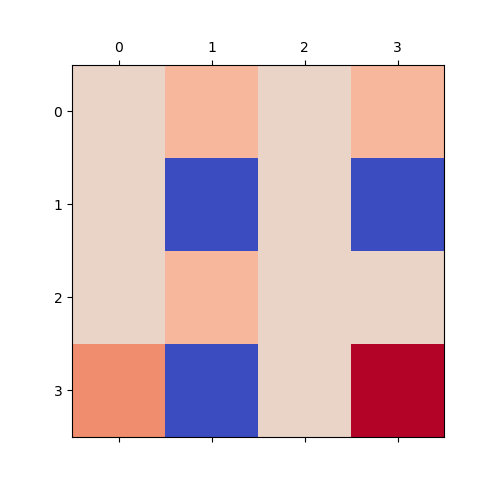
\includegraphics[width=3in]{0.png}
\caption{Reward result.}\label{fig1}
\end{figure}

Now we are ought to help it learn from the reward matrix, thus it can eat the cheese on the $(3,3)$ and avoid traps on $(1,1)$, $(1,3)$ and $(3,1)$. Recall the \emph{Q-learning} you learned from class, the mouse itself has to build a Q-table $Q(s,a)$ where $s$ is the state and $a$ is the action, then it can decide which action to take by this Q-table. Updating this Q-table is commonly performed as algorithm \ref{alg1}:

\begin{algorithm}[b] 
\caption{Q table learning \label{alg1}} %算法的名字
\hspace*{0.02in} {\bf Input:} %算法的输入, \hspace*{0.02in}用来控制位置,同时利用 \\ 进行换行
Initialize $Q(s,a)$ arbitrarily
\begin{algorithmic}[1]
\For{for each episode}
\State Initialize $s$
\While{$s$ is not terminal}
\State Choose $a$ from $s$ using policy derived from $Q$ (e.g., $\epsilon$-greedy)
\State Take action $a$, observe $r$, $s^{\prime}$
\State $Q(s,a) \gets Q(s,a) + \alpha \left ( r + \gamma \max_{a^{\prime}}Q(s^{\prime},a^{\prime}) - Q(s,a) \right )$
\State $s\gets s^{\prime}$
\EndWhile
\EndFor
\end{algorithmic}
\end{algorithm}
This algorithm includes hyper parameters as $\epsilon$, $\alpha$ and $\gamma$. The $\epsilon$ here is used for $\epsilon$-greedy strategy, which means during learning, the mouse has $\epsilon$ probability to randomly select an action, or it will select the action with best expected reward; $\gamma$, $\alpha$ are discounted rate and learning rate, respectively.

In this homework, you are only required to achieve the \emph{do} and \emph{learn} functions of the mouse. \textbf{There are several rules need to be noted}:
\begin{enumerate}
\item The mouse at most has \textbf{4} alternative actions: left, rigth, up, down, and when it is at the boundary of the grid, it cannot jump out of it.

\item The terminal condition for learning at each step is that the mouse succeeds to eat the largest cheese (reward = 4) or the mouse is trapped (reward = -5).

\item Each cheese can at most be eaten once. That is, after the mouse passes by, the reward becomes 0.

\end{enumerate}


\begin{flushleft}
\hrule
You are encouraged to achieve the following 2 extra questions if you are interested in reinforcement learning (RL).
Please save the code for the two extra questions in a different file from the code for the question \ref{q1}.
\hrule
\end{flushleft}


\question (Extra Credits, 2 points)  If you have compeleted the question \ref{q1}, can you quantitatively analyze the value distribution of the learned Q-table, such as drawing a matrix which consists of average estimated reward of four actions at each point. Then, evaluate the mean squared error (MSE) between the learned Q-table and the real reward matrix, and analyze which place these two matrices are most different, and try to give your explanation.

\question (Extra Credits, 4 points)  In practice, we often use what is called \emph{Deep Q-learning} instead of simple Q-table learning. That is, we use a deep neural network to fit the Q-table, with the current state of the agent as its inputs. Then the decision is made by ranking the output of the deep neural network. Can you design a neural network, and perform Deep Q-learning on the given reward matrix named \textbf{reward\_10\_10.npy} ? After that, compare the performance of Deep Q-learning and Q-table learning on this $10\times 10$ grid, show your results and analysis in a pdf and submit it. (Tip: You can use \textbf{pytorch} or \textbf{tensorflow} to build a deep neural network easily.)


\end{questions}


\begin{flushleft}
\textbf{Notice for the question \ref{q1}}: \\
\begin{enumerate}
\item You are ought to perform $\epsilon$-greedy, forbid the mouse jumping out of grid as well as ensure the mouse succeeding to reach $(3,3)$ at last in evaluation step. The correctness of implementation will be taken into account for scoring.
\item Submit your codes and the results in image or pdf.
\item \textbf{DO NOT} change other part of codes apart from the given spaces for you to fill, the parameters are carefully tuned in advance.
\item The final result would be like Fig.\ref{fig1} if your code is right.




\begin{figure}[htbp]
\centering
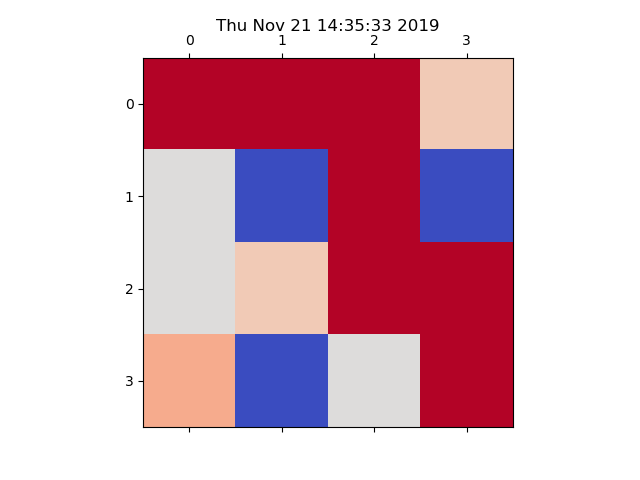
\includegraphics[width=4in]{1.png}
\caption{Trajectory result.}\label{fig2}
\end{figure}

\end{enumerate}
\end{flushleft}


\bibliographystyle{plain}
\bibliography{ref}

\end{document}
%%% Local Variables:
%%% mode: latex
%%% TeX-master: t
%%% End:

%  LocalWords:  headandfoot covariance
